Some research studies have been conducted on the practices that this thesis involves. In this chapter related works will be acknowledged.

\section{Spatiotemporal information from urban systems}
In the novel study of "Detecting flu outbreaks based on spatiotemporal information from urban system", which is the base idea for this thesis, Grottenberg et al. \cite{spatiotemp_urban_sys} outlines a design for a system for surveillance of flu outbreaks. Emphasis on the belief that real-time data flows could prove useful in both understanding social functions during disasters and crisis as well as give " ... actionable intelligence for use in influenza management efforts.".
The borrowed figure \ref{fig:grottenberg} from his article sums up what this thesis hopes to accomplish, namely to find a correlation between different datasets and the datasets from the Norwegian public health institution (NIPH), this interference of public behaviour would become visible in essential criterion.
This short read \cite{spatiotemp_urban_sys} is recommended as it gives a more in-depth understanding of the incentive for this thesis

\begin{figure}[h]
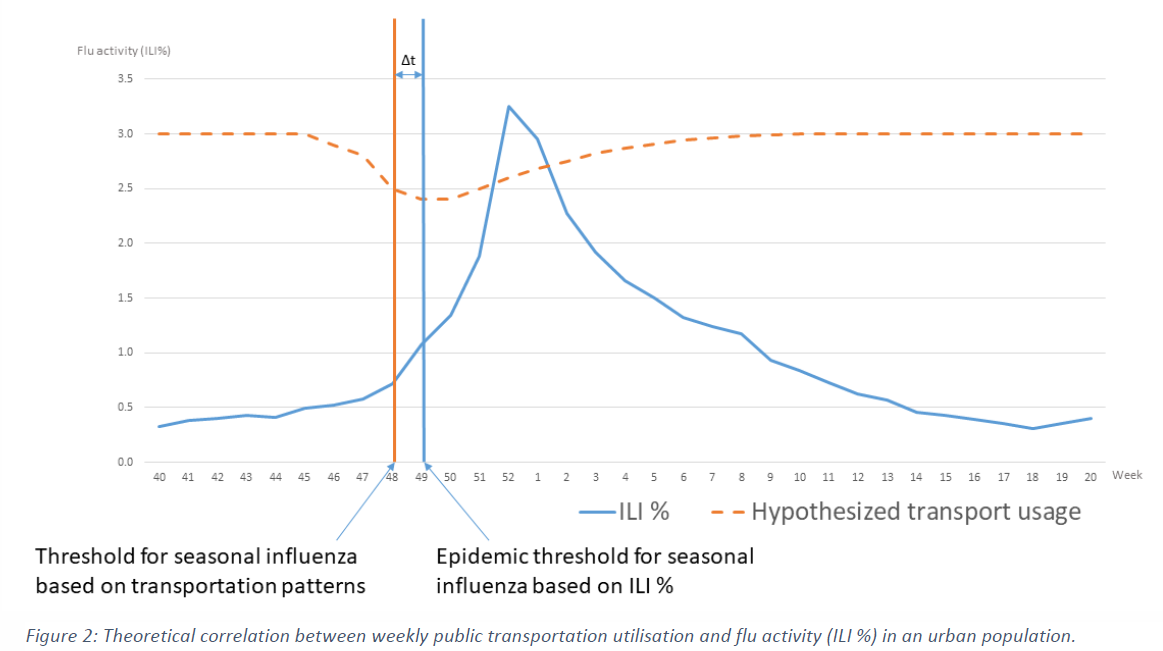
\includegraphics[width=16cm]{grottenberg}
\centering
\caption{Figure from Grottenberg et al. \cite{spatiotemp_urban_sys}}
\label{fig:grottenberg}
\end{figure}




\section{Twitter}
A number of studies have been created on the information users on Twitter generate in providing valuable insights into the population by analysing millions of twitter messages (tweets). Researchers have studied tweets to reveal political opinions\cite{twitter_politic}, measure public health\cite{twitter_flu_trends}, linguistic sentiments\cite{twitter_linguistics} and even environmental phenomena such as earthquakes\cite{twitter_earthQuake}. Achrekar et al.\cite{twitter_flu_trends} examines tweet flu trends and compares them with actual influenza data. The results show a high correlation between self-reported instances of flu-like illnesses (ILI) and reported ILI by public health providers. Achrekar references claims that early prevention limits the spread of infectious diseases and that twitter data is an 'untapped data source' that actually is quite reliable. This demonstrates how social media can be  used to predict real-world consequences, and gives credibility to usage in this thesis. \\Michal J. Paul and Mark Dredze \cite{twitter_what_you_tweet} also conducted research on the usage of twitter data to measure population characteristics. In their conclusion twitter data from many users divulges reliable information about a certain topic of interest and in particular public health. They further discuss the pros and cons namely that self-reported is low cost and rapid transmission, whereas on the other side this is a 'blind authorship, lack of source citation and presentation of opinion as fact'. Certainly twitter messages may be false on an individual level, but however when taking into account thousands or even millions of messages this seems not plausible on a bigger scale. For these reasons twitter data is used in this thesis as it proves an interesting and unique source of relevant information.